\section{Arquitecturas propuestas}\label{sec:arch}

Muchos son los sistemas de recuperación de información geográfica que han sido
propuestos. En las siguientes secciones se analizará tanto la arquitectura
básica de estos sistemas así como algunas de las propuestas más avanzadas.

\subsection{Arquitectura básica}\label{sec:archbas}

\begin{figure}[htb]%
	\begin{center}
		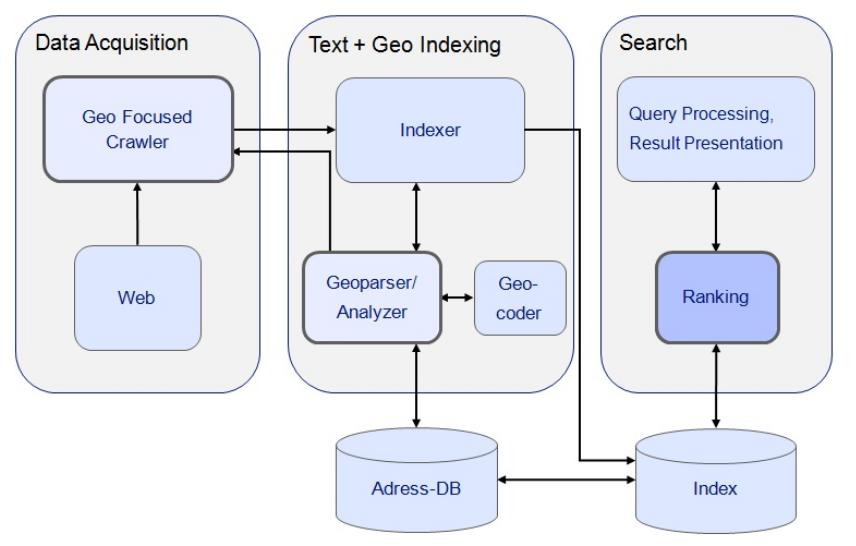
\includegraphics[width=0.8\textwidth]{basic_arch.jpg}
	\end{center}
	\caption{Arquitectura básica de un sistema de RIG \cite{cai2011}}
	\label{fig:archbas}
\end{figure}

Como se puede apreciar en la figura \ref{fig:archbas}, la arquitectura básica
de un sistema de RIG consta de 3 estapas principales: adquisición de de datos,
indexado y finalmente la búsqueda o recuperación de información. En la primera
etapa se utilizan \emph{crawlers} enfocados directamente a extraer información
geográfica de la web. Muchas de las fuentes no tienen los datos de forma
estructurada, es por ello que en la segunda etapa mucha de la información es
analizada y parseada. En esta estapa es donde la información de guarda en la
base de datos e indexada. En la tercera etapa, al realizar la búsqueda de la
información, la misma pasa por un proceso de \emph{ranking} o evaluación. Esto
permite que se pueda encontrar la información más relevante de una forma más
eficiente.

\clearpage

\subsection{SPIRIT}\label{sec:archspirit}

\begin{figure}[htb]%
	\begin{center}
		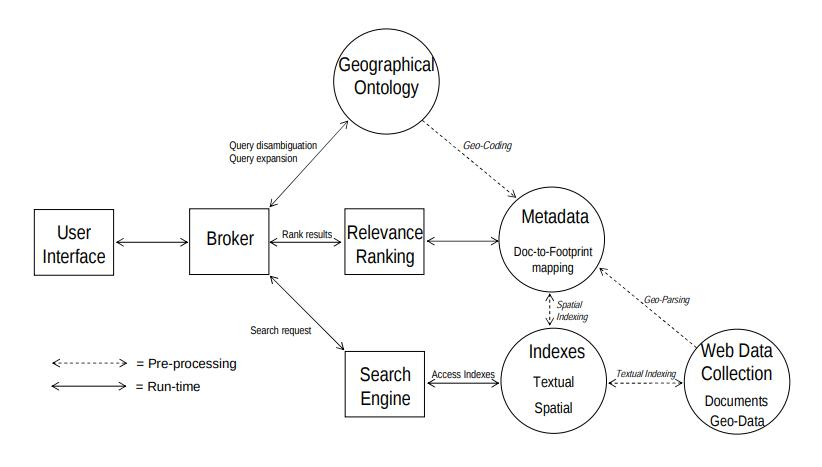
\includegraphics[width=0.8\textwidth]{spirit_arch.jpg}
	\end{center}
	\caption{Arquitectura de SPIRIT \cite{purves2007}}
	\label{fig:archspirit}
\end{figure}

En esta propuesta el trabajo de \cite{purves2007} describe el diseño,
implementación y evaluación de un motor de búsqueda de información geográfica
el cual es capaz de realizar búsquedas en forma de tripletas: tema - relación
espacial - locación. Como se puede ver en la figura \ref{fig:archspirit}, los
documentos además de ser indexados y almacenados en una base de datos, tambén
se les agrega un \emph{footprint} lo cual permite que se pueda identificar y
relacionar de forma más precisa la información.

En este sistema se aplicaron métodos para la búsqueda y exploración de los
resultados los cuales se evalúan en cuanto a su relevancia teniendo en cuenta
la temática y además la relación espacial de los mismos. Se hace uso también de
ontologías geográficas para la desambiguación de las búsquedas hechas por los
usuarios. Se muestran además dos formas de indexar la información: textual y
espacial. La primera forma de indexar (textual) se realiza directamente del
conjunto de documentos, la segunda forma (espacial) se puede apreciar en la
figura \ref{fig:archspirit} que se realiza utilizando los metadatos agregados a
los documentos.

\clearpage

\subsection{GeoUJA}\label{sec:archgeouja}

\begin{figure}[htb]%
	\begin{center}
		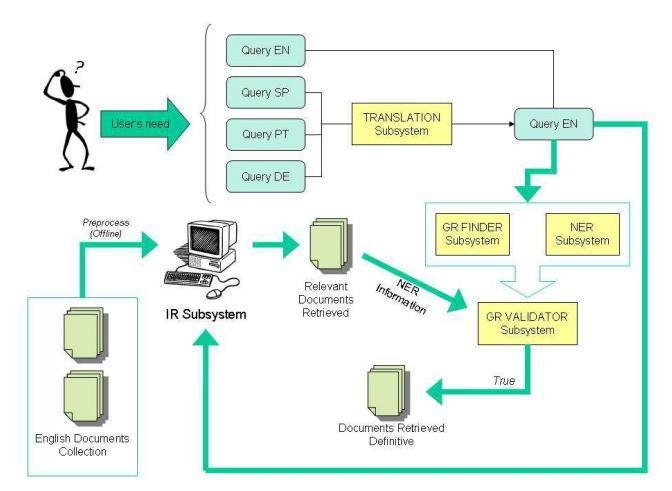
\includegraphics[width=0.8\textwidth]{geouja_arch.jpg}
	\end{center}
	\caption{Arquitectura de GeoUJA \cite{perea2007}}
	\label{fig:archgeouja}
\end{figure}

GeoUJA \cite{perea2007} es un sistema de RIG presentado por un grupo de la
Universidad de Ja'en en el evento GeoCLEF 2007. La arquitectura de este sistema
se basa en cinco módulos (o subsistemas) principales como se puede apreciar en
la figura \ref{fig:archgeouja}. Los módulos son: subsistema de recuperación de
información, subsistema de traducción, subsistema de búsqueda de relaciones
geográficas, subsistema de reonocimiento de nombres de entidades y subsistema
de validación.

Primeramente el usuario ingresa una búsqueda (en cuatro posibles idiomas) la
cual, en caso de ser necesario se traduce al inglés utilizando el susbsistema
de traducción, y se envía al subsistema de recuperación de información para
extraer los documentos relevantes. Esta búsqueda es también procesada por los
subsistemas de búsqueda de relaciones geográficas y reconocimiento de nombres de
entidades. Luego de este preprocesamiento, y en conjunto con los documentos
relvantes extraídos previamente, se realiza un validación de los mismos y se
devuelve al usuario un conjunto de documentos que el sistema en general
clasifica como relevantes.

\clearpage

\subsection{GeoFinder}\label{sec:archgeofinder}

\begin{figure}[htb]%
	\begin{center}
		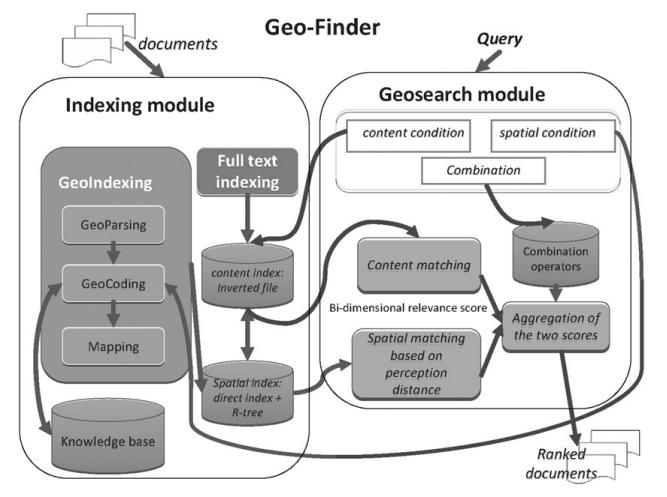
\includegraphics[width=0.8\textwidth]{geofinder_arch.jpg}
	\end{center}
	\caption{Arquitectura de GeoFinder \cite{bordogna2012}}
	\label{fig:archgeofinder}
\end{figure}

Otra arquitectura interesante a presentar es la que propone GeoFinder
\cite{bordogna2012}. En la misma se divide el proceso en dos módulos principales
como se puede apreciar en la figura \ref{fig:archgeofinder}. El primer módulo es
el encargado de indexar los documentos. En este es donde se realiza la
\emph{estructuración} de los documentos (\emph{geo-indexing}) y se almacenan.
En el segundo módulo se realiza la búsqueda de la información.

Al realizar una búsqueda, la misma se utiliza para buscar documentos
relacionados por el contenido y documentos relacionados espacialmente. Luego,
los documentos se evalúan teneiendo encuenta estas dos formas antes mencionadas
(contenido y espacio). Finalmente teniendo en cuenta ambas métricas los
resultados se combinan para extraer la mejor selección de documentos.

\clearpage

